\section{ROM-OpInf}

\begin{frame}{Operator Inference (OpInf)}
\begin{center}
    OpInf is a \textbf{data-driven}, \textbf{non-intrusive} ROM.
\end{center}

\vspace{0.3cm}

    \begin{description}
    \item[\textbf{Data-driven}:] Only high-fidelity snapshot data required ($\mathbf{Q}$).\vspace{0.1cm}
    %\item[\textbf{Projection-based}:] Projects FOM operators and states onto low-dim. subspace ($\mathbf{V}_r$).\vspace{0.1cm}
    \item[\textbf{Non-intrusive}:] No access needed to the underlying full-order governing equations.
    \end{description}

\vspace{0.6cm}

\textbf{Example}: 1D - Burgers' Eq.
$$\dfrac{\partial}{\partial t}q(x,t) = \nu\dfrac{\partial^2 }{\partial x^2}q(x,t) - \dfrac{\partial }{\partial x}\dfrac{q(x,t)^2}{2} ~~ \xLongrightarrow{Discret. + MOR} ~~  \dot{\hat{\mathbf{q}}}(t) = \hat{\mathbf{A}}\hat{\mathbf{q}}(t) + \hat{\mathbf{H}}\left(\hat{\mathbf{q}}(t)\otimes\hat{\mathbf{q}}(t) \right).$$

We infer $\hat{\bm{\theta}}=[\hat{\mathbf{A}},\hat{\mathbf{H}}]\in\mathbb{R}^{r\times(r+r^2)}$ by: $~\displaystyle\min_{\hat{\bm{\theta}}} \sum_{i=1}^k\Bigg\| \left[\hat{\mathbf{A}}\hat{\mathbf{q}}(t_i) + \hat{\mathbf{H}}\left(\hat{\mathbf{q}}(t_i)\otimes\hat{\mathbf{q}}(t_i) \right)\right] - \dot{\hat{\mathbf{q}}}(t_i)\Bigg\|_2^2$.

\end{frame}


\begin{frame}{Training Reduced Operators - Inference Process}
    \vspace{0.2cm}
    \centering
    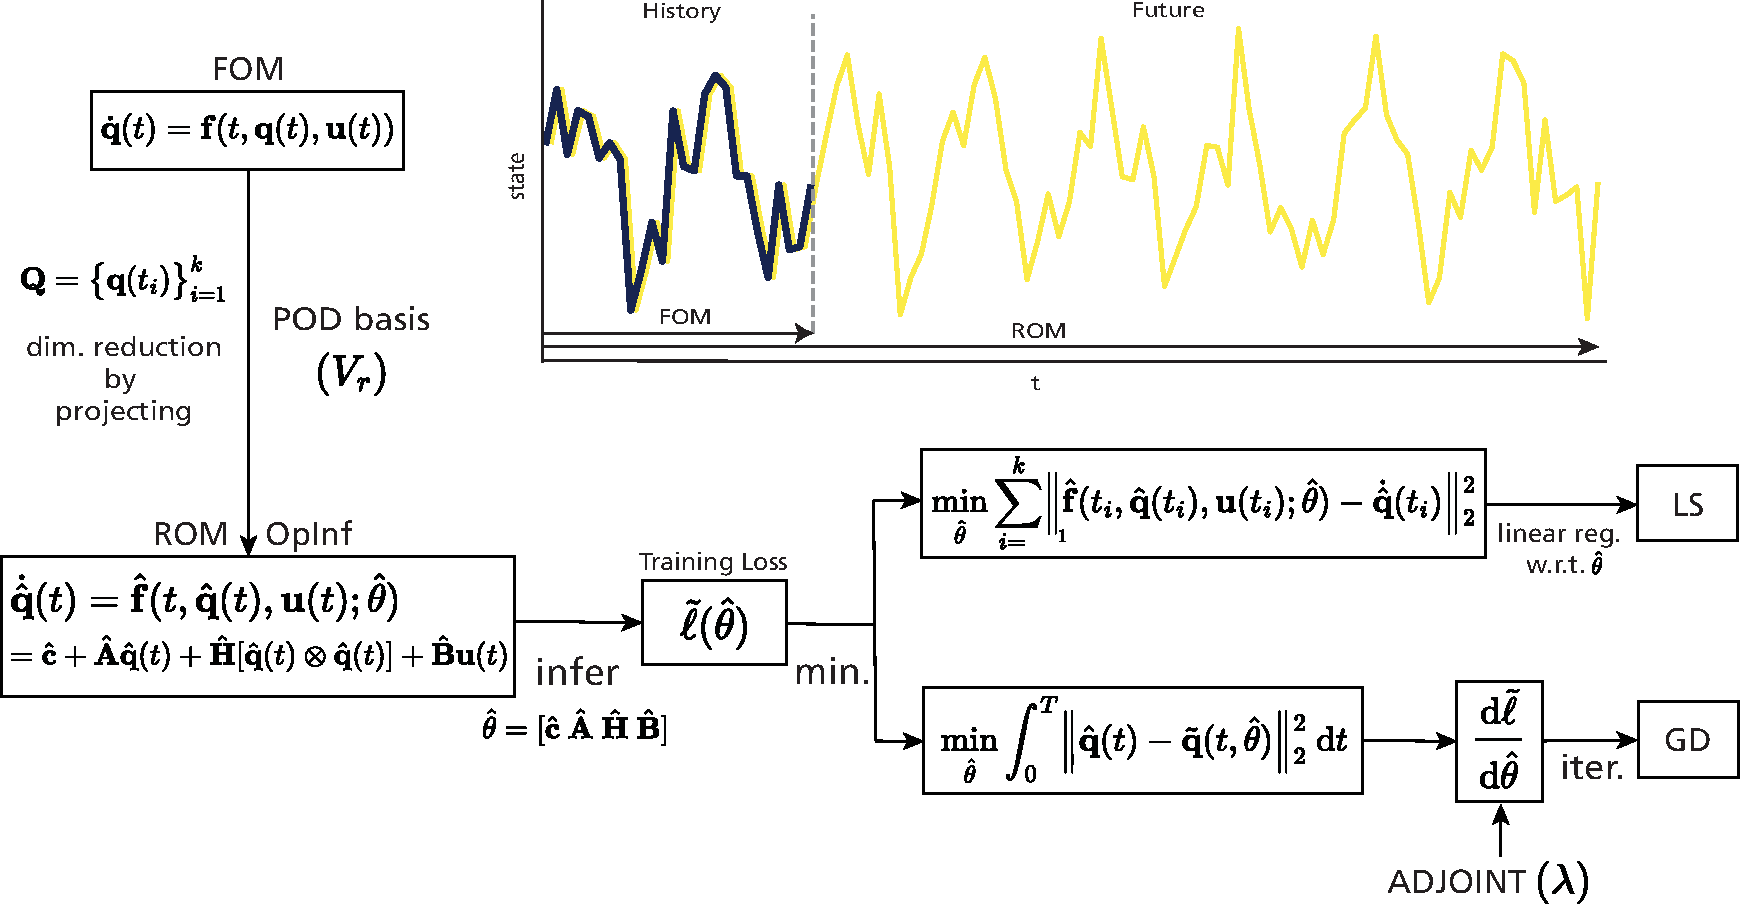
\includegraphics[width=0.97\textwidth]{images/intro_scheme.pdf} 
    %\caption{Caption for the image}
\end{frame}